\documentclass[11pt,a4paper]{article}

\usepackage[utf8]{inputenc}
\usepackage[T1]{fontenc}
\usepackage[margin=2.5cm]{geometry}
\usepackage{amsmath,amssymb}
\usepackage{booktabs}
\usepackage{array}
\usepackage{longtable}
\usepackage[l3]{csvsimple}
\usepackage{graphicx}
\graphicspath{{report/}{./}}
\usepackage{float}
\usepackage{pdflscape}
\usepackage{caption}
\usepackage{xcolor}
\usepackage{textcomp}
\usepackage{enumitem}
\usepackage{hyperref}
\usepackage{microtype}
\usepackage{qrcode}

\hypersetup{
  colorlinks=true,
  linkcolor=blue!50!black,
  citecolor=blue!50!black,
  urlcolor=blue!60!black,
  pdftitle={FIN42350 Portfolio Design Project},
  pdfauthor={Mina Youssef}
}

\setlength{\parindent}{0pt}
\setlength{\parskip}{0.55em}
\setlist[itemize]{noitemsep,topsep=0.3em}
\setlist[enumerate]{noitemsep,topsep=0.3em}

\newcommand{\EUR}{\texteuro}
\newcommand{\todo}[1]{\textcolor{red!70!black}{[TODO: #1]}}
\newcommand{\placeholder}[2][0.92\linewidth]{%
  \begin{center}
    \fbox{\parbox[c][#2][c]{#1}{\centering Figure placeholder}}
  \end{center}
}

\title{FIN42350 Capital Markets - Group Project\\
\large A Systematic Framework for Client-Specific Portfolio Construction and Risk Analysis}
\author{Student Name: Mina Youssef\\Student Number: 14200381}

\begin{document}
\hypersetup{pageanchor=false}

\begin{titlepage}
  \thispagestyle{empty}
  \centering
  \vspace*{0.8cm}

  
\includegraphics[width=0.76\textwidth]{ucd-smurfit-logo.png}

  \vfill

  {\color{blue!50!black}\rule{0.82\textwidth}{1.5pt}}\\[1.2cm]
  {\Huge\bfseries FIN42350 Capital Markets\\[0.35cm] Group Project\par}
  \vspace{0.9cm}
  {\LARGE A Systematic Framework for Client-Specific\\[0.25cm] Portfolio Construction and Risk Analysis\par}
  \vspace{1.2cm}
  {\color{blue!50!black}\rule{0.82\textwidth}{1.5pt}}

  \vfill

  {\Large\textbf{Student Name:} Mina Youssef\par}
  \vspace{0.3cm}
  {\Large\textbf{Student Number:} 14200381\par}

  \vfill

  {\large UCD Michael Smurfit Graduate Business School\par}
  \vspace{0.2cm}
  {\large University College Dublin\par}
  \vspace{0.5cm}
  {\large October 2026\par}
\end{titlepage}

\clearpage
\thispagestyle{empty}
\begin{center}
  \vspace*{1cm}
  {\Huge\bfseries Project Resources\par}
  \vspace{0.4cm}
  {\large Scan the QR codes to access the live application and complete project repository.\par}

  \vspace{1.3cm}
  {\Large\bfseries Live Streamlit Application\par}
  \vspace{0.45cm}
  {\color{black}\qrcode[height=4.5cm]{https://fin42350-capital-market-group-project.streamlit.app}}
  \vspace{0.35cm}

  \href{https://fin42350-capital-market-group-project.streamlit.app}{\texttt{fin42350-capital-market-group-project.streamlit.app}}

  \vspace{1.2cm}
  {\Large\bfseries GitHub Repository\par}
  \vspace{0.45cm}
  {\color{black}\qrcode[height=4.5cm]{https://github.com/minavyoussef/FIN42350-Capital-Market-Group-Project}}
  \vspace{0.35cm}

  \href{https://github.com/minavyoussef/FIN42350-Capital-Market-Group-Project}{\texttt{github.com/minavyoussef/FIN42350-Capital-Market-Group-Project}}
\end{center}

\clearpage
\hypersetup{pageanchor=true}
\pagenumbering{roman}
\begingroup
  \footnotesize
  \setlength{\parskip}{0pt}
  \tableofcontents
\endgroup

\clearpage
\pagenumbering{arabic}

\begin{abstract}
  This report develops a systematic framework for constructing a multi-asset portfolio based on an investor specific preference. The frame has been designed into five phases using in-sample historical data for portfolio allocation and out-of-sample data for the optimised portfolio performance evaluation. In addition, we use Monte Carlo simulation future expected return under three different investor profiles, risky, balanced, and conservative with SPY as a proxy for market benchmark.
\end{abstract}
\newpage

% Target: approximately 3,000 words, excluding appendices.

% =============================================================================
\section{Introduction}
\label{sec:introduction}

We present an end-to-end systematic framework for multi-asset portfolio design and construction. Conceptually, we distinguish the design process into two decision layers. The first layer determine asset allocation based on investor risk aversion profile score, while second layer optimise securities allocation within each asset class.

We begin with an overview of \hyperref[sec:methodology]{Portfolio Design and Construction Process}, describing the end-to-end approch that has been designed. The framework comprises into five main phases. \hyperref[sec:phase-one]{Phase I --- Investor Profile and Risk Assessment}, examing main investor questionnaire, the importance assigned to each question as weight, and calculation of risk score. \hyperref[sec:phase-two]{Phase II --- Investor Suitability and Asset-Class Allocation}, we discuss the first decision layer of main asset class allication based on predified asset suitability lookup approach. \hyperref[sec:phase-three]{Phase III --- Market Data Preparation}, we examin dataset construction, including currency conversion, annualised return calculation, and muti-assets variance/co-variance matrix creation. \hyperref[sec:phase-four]{Phase IV --- Portfolio Optimisation} combines historical data preparation, investor risk aversion coefficient, asset class allocations proportions and optimise the exact allication percentage wihin each of the the asset class instruments for optimial performance. Finally, \hyperref[sec:phase-five]{Phase V --- Portfolio Benchmarking and Performance Analysis}, evaluate the proposed portfolio using out-of-sample period, an EUR-denominated S\&P 500 benchmark, Value at Risk (VaR) and Expected Shortfall (ES), and Monte Carlo simulation. The simulation estimates the distribution of possible outome under physical market measurement.

The \hyperref[sec:concrete-run]{Concrete Client Run and Results}, demonstrates how the framework converts investor information and historical market data into an implementable portfolio recommendation.

The report concludes with the \hyperref[sec:conclusion]{Conclusion}, which summarises the principal findings, limitations, and final portfolio recommendation.

% =============================================================================
\section{Portfolio Design and Construction Process}
\label{sec:methodology}

In this section we give an overview of the design and the main principles was held during this process. Figure \ref{fig:e2e-workflow} shows the end-to-end design steps.

\textit{\hyperref[sec:phase-one]{Phase I --- Investor Profile and Risk Assessment}} step begins with a set of questions designed to capture investor-specific characteristics. The investor's answers are then weighted according to the importance assigned to each question by the investor preference. The principle rationale for such decision, given two different investors profiles who provided identical responses but place different levels of importance on each question would recieve different risk scores and profile recommendations. Finally, the investor risk score is mapped to a risk-aversion coefficient, \(\lambda\), which serves as an input to the portfolio-weight optimisation in Phase IV.

\clearpage
\begin{landscape}
  \thispagestyle{plain}
  \begin{figure}[H]
    \centering
    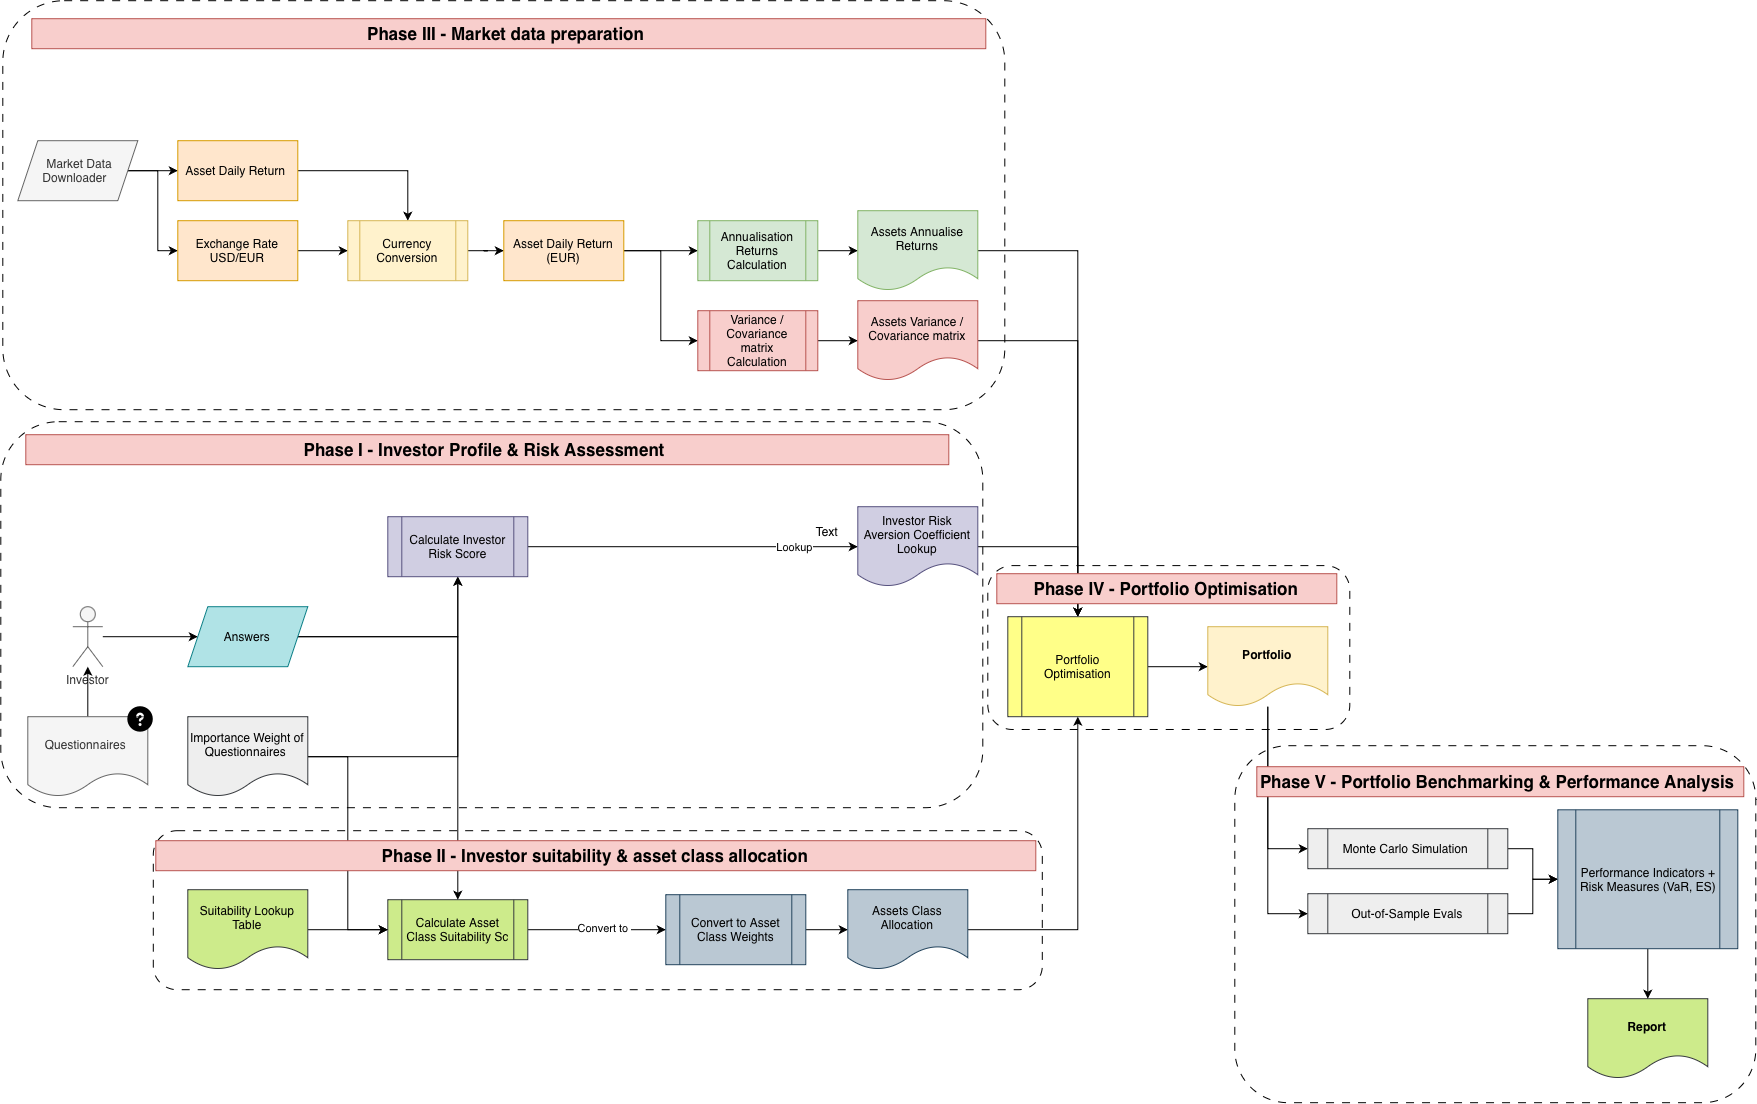
\includegraphics[
      width=0.96\linewidth,
      height=0.82\textheight,
      keepaspectratio
    ]{fig-1-e2e-framework-diagram.png}
    \caption{End-to-end portfolio construction and evaluation workflow}
    \label{fig:e2e-workflow}
  \end{figure}
\end{landscape}
\clearpage

\textit{\hyperref[sec:phase-two]{Phase II --- Investor Suitability and Asset-Class Allocation}} step main objective is to provide an allocation for each asset class basded on asset-class suitability score $S_c$. Calculating asset-class suitability score $S_c$ depneds on $(i)$ Investor's questionnaire importance weight $(ii)$ Asset class suitability lookup table. The output of this step will be feeding as a constraint into Phase IV - Portfolio Optimisation.

\textit{\hyperref[sec:phase-three]{Phase III --- Market Data Preparation}} step focus on retrieval financial market data from available data source, and adjusting the frequency of return, in our case daily we utilise Yahoo Finance and adjust for daily return. In addition, we retrieved USD/EUR exchange rate, and applying rate conversion on price action before return/annualised returns calculations. Finally, we construct variance-covariance matrix which serves as an input to the portfolio-weight optimisation in Phase IV.

\textit{\hyperref[sec:phase-four]{Phase IV --- Portfolio Optimisation}} step taking in calcuated variance-covariance metix $\Sigma$, asset class allocation vector $\vec{W}$, and investor risk aversion coefficient and optimise against allocation within asset class, producing taregt portfolio.

\textit{\hyperref[sec:phase-one]{Phase V --- Portfolio Benchmarking and Performance Analysis}} final phase focus is to conduct full assessment of the resultant portfolio. The assesment start with out-of-sample evaluation of 2-years, following a calcuation of set of performance indicators including, and finally we apply Monte Carlo simulation to produce expected potensional return given allocated assets expected return and variaiance.

In the following next sections, we discuss in-deepth each of the five phases and provide sample output as examples.

% =============================================================================
\section{Phase I --- Investor Profile and Risk Assessment}
\label{sec:phase-one}

We start by building the investor's profile and quantifying their risk aversion through risk aversion coefficient.

\subsection{Investor questionnaire and weights}

The investor is asked the questions presented in Table~\ref{tab:questionnaire-scale}. The discretisation of year ranges make the investment-horizon choices reproducible.

\begin{table}[H]
  \centering
  \small
  \caption{Investor questionnaire and five-level answer scales}
  \label{tab:questionnaire-scale}
  \begin{tabular}{>{\raggedright\arraybackslash}p{0.18\linewidth}>{\raggedright\arraybackslash}p{0.43\linewidth}>{\raggedright\arraybackslash}p{0.31\linewidth}}
    \toprule
    Attribute & Question presented to the investor & Five-level response range \\
    \midrule
    Risk tolerance & How much short-term loss could you tolerate without selling your investments? & Very low--Very high (5 levels) \\
    Investment horizon & When do you expect to begin using most of this investment? & Very short ($<1$ year); Short (1--3 years); Medium (3--5 years); Long (5--10 years); Very long ($>10$ years) \\
    Growth objective & How strongly do you prioritise long-term capital growth over current income? & Very low--Very high (5 levels) \\
    Capital preservation & How important is avoiding a loss of the amount initially invested? & Very low--Very high (5 levels) \\
    Liquidity requirement & How much of this portfolio might you need to withdraw at short notice? & Very low--Very high (5 levels) \\
    \bottomrule
  \end{tabular}
\end{table}

We attached an importance points for each of the Attribute defined, where the total sum of all the weight would be summed to 10, and thier normalised values summed equal to one.

Table~\ref{tab:questionnaire-example} provides an illustrative set of responses and investor-assigned importance points. The points sum to 10 and are normalised to weights that sum to one.

\begin{table}[H]
  \centering
  \scriptsize
  \setlength{\tabcolsep}{2pt}
  \caption{Illustrative questionnaire responses, importance weights, and answer normalisation}
  \label{tab:questionnaire-example}
  \begin{tabular}{>{\raggedright\arraybackslash}p{0.17\linewidth}>{\raggedright\arraybackslash}p{0.09\linewidth}>{\centering\arraybackslash}p{0.10\linewidth}>{\centering\arraybackslash}p{0.10\linewidth}>{\raggedright\arraybackslash}p{0.36\linewidth}>{\raggedright\arraybackslash}p{0.10\linewidth}}
    \toprule
    Attribute and key & Example answer & Importance points & Normalised weight & Values mapped from 0 to 1 & Direction \\
    \midrule
    0. Risk tolerance\newline\texttt{risk\_\allowbreak tolerance} & Moderate & 3 & 0.30 & Very low = 0; Low = 0.25; Moderate = 0.50; High = 0.75; Very high = 1 & Increasing \\
    1. Investment horizon\newline\texttt{investment\_\allowbreak horizon} & Long & 2 & 0.20 & Very short = 0; Short = 0.25; Medium = 0.50; Long = 0.75; Very long = 1 & Increasing \\
    2. Growth objective\newline\texttt{growth\_\allowbreak objective} & High & 2 & 0.20 & Very low = 0; Low = 0.25; Medium = 0.50; High = 0.75; Very high = 1 & Increasing \\
    3. Capital preservation\newline\texttt{capital\_\allowbreak preservation} & Medium & 2 & 0.20 & Very low = 1; Low = 0.75; Medium = 0.50; High = 0.25; Very high = 0 & Decreasing \\
    4. Liquidity requirement\newline\texttt{liquidity\_\allowbreak requirement} & Low & 1 & 0.10 & Very low = 1; Low = 0.75; Medium = 0.50; High = 0.25; Very high = 0 & Decreasing \\
    \midrule
    \multicolumn{2}{r}{Total} & 10 & 1.00 & & \\
    \bottomrule
  \end{tabular}
\end{table}

\subsection{Investor risk score and risk-aversion coefficient}

The normalised investor risk score $R_Q\in[0,1]$ quantifies the investor's risk profile and is mapped to the risk-aversion coefficient $\lambda$, as shown in Table~\ref{tab:risk-profile-lambda}.
\begin{equation}
  R_Q=\sum_{j=1}^{J}\alpha_jq_j,
  \qquad
  \sum_{j=1}^{J}\alpha_j=1,
\end{equation}
where $q_j\in[0,1]$ is the normalised answer and $\alpha_j$ is the question's importance weight.

\begin{table}[H]
  \centering
  \caption{Investor risk-score intervals, profiles, and risk-aversion coefficients}
  \label{tab:risk-profile-lambda}
  \begin{tabular}{lcr}
    \toprule
    $R_Q$ interval & Profile & $\lambda$ \\
    \midrule
    $[0.00, 0.20)$ & Very conservative & 12 \\
    $[0.20, 0.40)$ & Conservative & 8 \\
    $[0.40, 0.60)$ & Moderate & 5 \\
    $[0.60, 0.80)$ & Growth & 3 \\
    $[0.80, 1.00]$ & Aggressive & 1 \\
    \bottomrule
  \end{tabular}
\end{table}

Risk-aversion coefficient $\lambda$, is the used as a control variable of how strongly the portfolio optimiser penalise risk relative to expected return in Phase IV.

% =============================================================================
\section{Phase II --- Investor Suitability and Asset-Class Allocation}
\label{sec:phase-two}

The first decision layer, after we collect investor's questionnaire answers and importance points, would be to perform asset class allocation.
Two components are needed $(i)$ Investor's questionnaire importance weight $\alpha_j$, $(ii)$ Asset-suitability lookup $A_{j,k_j,c}\in[0,1]$.

\subsection{Asset suitability lookup}

The asset-suitability lookup is a predefined scoring table that translates an investor's questionnaire answers into suitability scores for each asset class.

For every combination of:
\[
  \text{Question} \times \text{Answer} \times \text{Asset class},
\]
the lookup assigns a score:
\[
  A_{j,k,c}\in[0,1],
\]
where:
\begin{itemize}
  \item \(j\) identifies the questionnaire question;
  \item \(k\) is the investor's selected answer;
  \item \(c\) identifies an asset class;
  \item \(A_{j,k,c}\) is the suitability score

\end{itemize}

And \(0\) means unsuitable and \(1\) means highly suitable.

For example, the complete risk-tolerance slice is shown in Table~\ref{tab:risk-tolerance-suitability}.

\begin{table}[H]
  \centering
  \caption{Risk-tolerance slice of the asset-suitability lookup}
  \label{tab:risk-tolerance-suitability}
  \begin{tabular}{lrrrrr}
    \toprule
    Risk tolerance & Equity & Fixed income & Cash & Real estate & Commodity \\
    \midrule
    Very low & 0.10 & 0.80 & 1.00 & 0.30 & 0.20 \\
    Low & 0.30 & 0.90 & 0.90 & 0.40 & 0.30 \\
    Moderate & 0.60 & 0.80 & 0.60 & 0.60 & 0.50 \\
    High & 0.85 & 0.50 & 0.30 & 0.75 & 0.70 \\
    Very high & 1.00 & 0.30 & 0.10 & 0.85 & 0.85 \\
    \bottomrule
  \end{tabular}
\end{table}

\subsection{Weighted asset-class suitability}

Arriving to the asset class weights that satisfies investor profile would require adjusting selected suitability score by investor answer's importance points for each asset class $S_c$.

\begin{equation}
  S_c=\sum_{j=1}^{J}\alpha_jA_{j,k_j,c}.
\end{equation}

where, $\alpha_j$ represents investoer's answer importance points, and $A_{j,k_j,c}$ representation asset-suitability lookup for question $j$, answer $k$, and asset class $c$.

Table~\ref{tab:asset-class-suitability-example} presents an example of the resulting suitability score for each asset class.

\begin{table}[H]
  \centering
  \caption{Illustrative asset-class suitability scores}
  \label{tab:asset-class-suitability-example}
  \begin{tabular}{clr}
    \toprule
    No. & Asset class & Suitability score \\
    \midrule
    0 & Equity & 0.730 \\
    1 & Fixed income & 0.705 \\
    2 & Cash & 0.545 \\
    3 & Real estate & 0.630 \\
    4 & Commodity & 0.550 \\
    \bottomrule
  \end{tabular}
\end{table}

\subsection{Conversion to asset-class weights}

In the final stage of the first decision layer, each asset-class suitability score, \(S_c\), is normalised to obtain its corresponding strategic asset-class weight, \(W_c\):

\begin{equation}
  W_c=\frac{S_c}{\sum_{c \in \mathcal{C}} S_c},
  \qquad
  \sum_{c \in \mathcal{C}} W_c=1,
\end{equation}

where \(\mathcal{C}\) denotes the set of eligible asset classes. This normalisation converts the suitability scores into proportional allocations that sum to one.

The resulting asset-class weight vector, \(\mathbf{W}\), is subsequently imposed as a set of constraints in the second decision layer, in which the optimiser determines the allocation among the eligible securities within each asset class.

% =============================================================================
\section{Phase III --- Market Data Preparation}
\label{sec:phase-three}

\subsection{Asset universe and market-data download}

The investable universe contains 134 instruments spanning nine asset classes, 78 asset subclasses, and 31 geographic classifications. Table~\ref{tab:usd-eur-rate-sample} show a head and tail sample of downloaded USD/EUR exchange rates. Table~\ref{tab:asset-universe-summary} summarises its composition, while Appendix~\ref{app:full-asset-universe} reports the complete instrument list. Full List of Asset universe are in Appendix~\ref{app:full-asset-universe}.

\begin{table}[H]
  \centering
  \caption{Sample of the daily USD/EUR exchange-rate series}
  \label{tab:usd-eur-rate-sample}
  \begin{tabular}{rrr}
    \toprule
    Observation & Date & USD/EUR rate \\
    \midrule
    0 & 2019-10-03 & 0.91210 \\
    1 & 2019-10-04 & 0.91113 \\
    2 & 2019-10-05 & 0.91113 \\
    3 & 2019-10-06 & 0.91113 \\
    4 & 2019-10-07 & 0.91020 \\
    \multicolumn{3}{c}{\ldots} \\
    2553 & 2026-09-29 & 0.87930 \\
    2554 & 2026-09-30 & 0.88177 \\
    2555 & 2026-10-01 & 0.88283 \\
    2556 & 2026-10-02 & 0.88830 \\
    2557 & 2026-10-03 & 0.88830 \\
    \bottomrule
  \end{tabular}
\end{table}

\begin{table}[H]
  \centering
  \caption{Summary of the investable asset universe}
  \label{tab:asset-universe-summary}
  \begin{tabular}{lrrr}
    \toprule
    Asset class & Instruments & Subclasses & Geographies \\
    \midrule
    Equity & 81 & 39 & 30 \\
    Fixed income & 19 & 11 & 3 \\
    Commodity & 15 & 12 & 1 \\
    Currency & 7 & 7 & 7 \\
    Volatility & 5 & 4 & 1 \\
    Real estate & 3 & 1 & 1 \\
    Crypto asset & 2 & 2 & 1 \\
    Cash & 1 & 1 & 1 \\
    Alternatives & 1 & 1 & 1 \\
    \midrule
    Total & 134 & 78 & 31 \\
    \bottomrule
  \end{tabular}
\end{table}

Yahoo Finance API are used as an endpoint to download market data. Total of 7 years of data were downloaded, with a chronological 5-years/2-years split for an in/out-of sample respectively.

\begin{table}[H]
  \centering
  \caption{Chronological in-sample and out-of-sample split}
  \label{tab:sample-periods}
  \begin{tabular}{lp{0.25\linewidth}p{0.50\linewidth}}
    \toprule
    Dataset & Period & Purpose \\
    \midrule
    Full sample & 3 Oct 2019--3 Oct 2026 & Full dataset (7 years) \\
    In-sample & 3 Oct 2019--2 Oct 2024 & Portfolio design and construction (5 years) \\
    Out-of-sample & 3 Oct 2024--3 Oct 2026 & Evaluate the frozen portfolio (2 years) \\
    \bottomrule
  \end{tabular}
\end{table}

\subsection{Currency conversion and EUR daily returns}

The exchange rate of USD/EUR were downloaded for the full period 7-years i.e. in/out-of sample, and applied conversion before calcuating daily return.

For a USD-denominated asset, we apply:

\begin{equation}
  P^{\mathrm{EUR}}_{i,t}
  =P^{\mathrm{USD}}_{i,t}X^{\mathrm{USD/EUR}}_t,
  \qquad
  r^{\mathrm{EUR}}_{i,t}
  =\frac{P^{\mathrm{EUR}}_{i,t}}{P^{\mathrm{EUR}}_{i,t-1}}-1.
\end{equation}

\subsection{Annualised return estimates}

Following daily return calcuation in EUR, annulaised return are calcuated to express an investement's return on a one-year bases. This would facilitate assessing level of investment horizon especially for longer term period.

\begin{equation}
  \hat\mu_i=252\,\bar r_{i,d}.
\end{equation}

\subsection{Variance and covariance estimates}

A variance-covariance matrix is calcuated out of annualised return $\hat{\Sigma}$, where it will be used as part of asset allocation with class in Phase IV.

\begin{equation}
  \hat\Sigma=252\,\operatorname{Cov}(r_d),
  \qquad
  \hat\sigma_i=\sqrt{\hat\Sigma_{ii}}.
\end{equation}

% =============================================================================
\section{Phase IV --- Portfolio Optimisation}
\label{sec:phase-four}

Phase IV represents the second decision layer of the portfolio design framework. In this phase, the optimiser determines how each assets are allocated within each asset class.

\subsection{Optimiser inputs}

The optimiser combines five inputs produced by the preceding phases:

\begin{enumerate}
  \item the annualised expected EUR return vector, \(\hat{\boldsymbol{\mu}}\);
  \item the annualised EUR return covariance matrix, \(\hat{\boldsymbol{\Sigma}}\);
  \item the investor's risk-aversion coefficient, \(\lambda\);
  \item the required asset-class weights, \(W_c\); and
  \item the set of eligible ETFs within each asset class.
\end{enumerate}

\subsection{Mean--variance objective}

The optimiser objective function select ETF weights that maximise the portfolio's expected return penalising overall variance. Using investoer's risk aversion coefficient $\lambda$ as a controlling coefficient.

A high investor's risk available coefficient $\lambda$ would result in greater emphasis on reducing the overall portfolio variance and therefore favours less risky allocation, and true vice versa.

\begin{equation}
  \max_w\left(
    w^{\top}\hat\mu-
    \frac{\lambda}{2}w^{\top}\hat\Sigma w
  \right).
\end{equation}

\subsection{Portfolio constraints}

\begin{align}
  \sum_i w_i &= 1, \\
  w_i &\geq 0, \\
  \sum_{i\in c}w_i &= W_c, \\
  w_i &\leq u_i.
\end{align}

The portfolio is subject to four principal constraints:

First, short selling is prohibited, so each ETF weight must be non-negative. Second, the summation of all ETFs within same asset class should be equal to the pre-defined asset class allocated weight $W_c$, that was defined in the first layer decision. Third, the profile must be fully invested. Finally, an upper limit is imposed to reduce concentration risk.

\subsection{Portfolio output and validation}

The in sample optimisation yield a fully investment portfolio with asset being allocated based on investor's risk aversion preference. Example of such allocation in Table~\ref{tab:sample-optimized-allocation}.

\begin{table}[H]
  \centering
  \scriptsize
  \caption{Sample optimised portfolio allocation}
  \label{tab:sample-optimized-allocation}
  \setlength{\tabcolsep}{3.5pt}
  \resizebox{\linewidth}{!}{%
    \begin{tabular}{p{0.31\linewidth}llp{0.18\linewidth}rr}
      \toprule
      Display name & Investment type & Geography & Asset type & Allocation (\%) & Allocation (\EUR) \\
      \midrule
      SPDR Bloomberg 1--3 Month T-Bill ETF & ETF & United States & Treasury bills & 17.25 & 172,468.35 \\
      VanEck Semiconductor ETF & ETF & Global & Semiconductors & 15.00 & 150,000.00 \\
      Schwab US TIPS ETF & ETF & United States & Inflation-linked bonds & 15.00 & 150,000.00 \\
      Real Estate Select Sector SPDR Fund & ETF & United States & Listed real estate & 15.00 & 150,000.00 \\
      United States Brent Oil Fund & ETF & Global & Brent crude oil & 7.34 & 73,444.30 \\
      iShares TIPS Bond ETF & ETF & United States & Inflation-linked bonds & 7.31 & 73,101.27 \\
      iShares Semiconductor ETF & ETF & United States & Semiconductors & 4.94 & 49,421.29 \\
      Vanguard Real Estate ETF & ETF & United States & Listed real estate & 4.94 & 49,367.09 \\
      iShares Silver Trust & ETF & Global & Silver & 4.93 & 49,342.22 \\
      Global X MSCI Argentina ETF & ETF & Argentina & Country equity & 3.16 & 31,591.37 \\
      Invesco DB Agriculture Fund & ETF & Global & Agriculture & 2.81 & 28,055.50 \\
      iShares Gold Trust & ETF & Global & Gold & 1.72 & 17,227.97 \\
      United States Copper Index Fund & ETF & Global & Copper & 0.60 & 5,980.65 \\
      \midrule
      Total & & & & 100.00 & 1,000,000.00 \\
      \bottomrule
    \end{tabular}
  }
\end{table}

\begin{figure}[H]
  \centering
  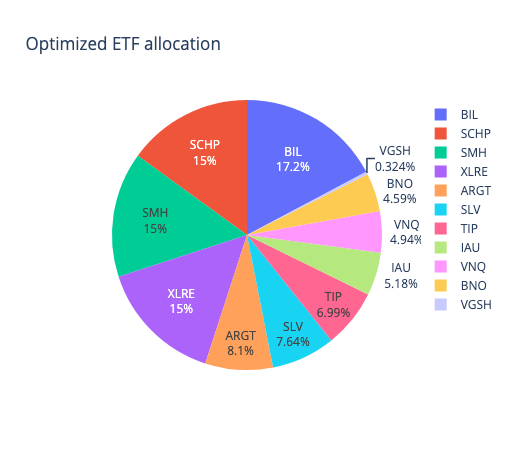
\includegraphics[width=0.9\linewidth]{optimized-etf-allocation.png}
  \caption{Sample optimised allocation of the \EUR1 million portfolio}
  \label{fig:sample-optimized-allocation}
\end{figure}

% =============================================================================
\section{Phase V --- Portfolio Benchmarking and Performance Analysis}
\label{sec:phase-five}

The final phase perform set of evaluations on the optimised portfolio, we start with benhmark calcification with out-of-sample of 2-years using S\&P 500 as a proxy to the market. Following we calculate Value at Risk (VaR) and Expected Shortfall (ES) at the 95$\%$ and 99$\%$ confidence levels. Finally, we apply Monte Carlo simulation to produce expected potensional return given allocated assets expected return and variaiance.

\subsection{Benchmark and out-of-sample evaluation}

The optimised portfolio weights were estimated exclusive in-sample data. subsequently, we apply benchmark on the out-of-sample portion of the dataset measuring the overall performance for the 2-years without rebancing.

An initial capital of €1 million would be allocated based on the produced weights, following by daily return calculating for each trading day based on the adjusted closing price. Since both the portfolio and benchmark contain US-dollar-denominated securities, their adjusted prices were converted into euros using the corresponding daily USD/EUR exchange rate, which was handled in Phase III - Market Data Prepration.

SPY was selected as the benchmark reflecting the market as a whole. The cumulative value of the portfolio and benchmark was calculated from the same initial investment:

\[
  V_t = V_0 \prod_{\tau=1}^{t}(1+r_\tau),
\]

where \(V_0\) is the initial capital and \(r_\tau\) is the daily euro-denominated return. A visualisation of the benchmark is shown in Figure~\ref{fig:out-of-sample-growth}.

\begin{figure}[H]
  \centering
  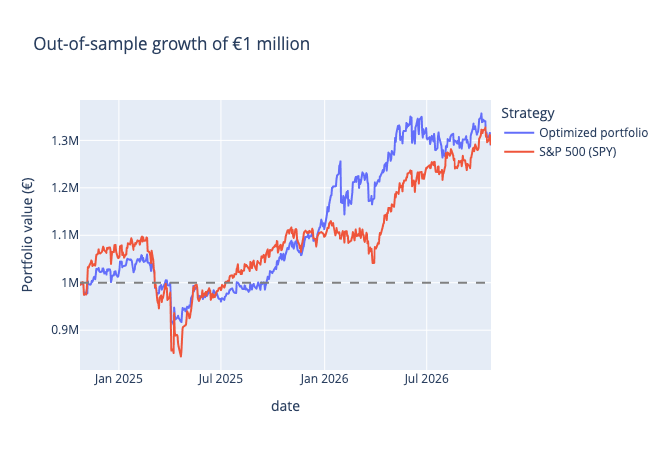
\includegraphics[width=0.9\linewidth]{out-of-sample-growth-of-1-million.png}
  \caption{Out-of-sample growth of the optimised portfolio and S\&P 500 benchmark from an initial investment of \EUR1 million}
  \label{fig:out-of-sample-growth}
\end{figure}

\subsection{Performance indicators}

Portfolio performance was evaluated starting with arithmatic average return, geometic average return, Risk-adjusted performance was assessed using the Sharpe ratio, which relates excess return to total volatility, and the Treynor ratio, which relates excess return to systematic risk measured by beta. Jensen’s alpha was used to identify returns exceeding those predicted by the CAPM, given the portfolio’s market exposure. The information ratio measures alpha relative to residual risk, or tracking error, while the \(M^2\) measure expresses Sharpe-based performance as an easily interpreted differential return relative to the market benchmark. Beta and \(R^2\), estimated against SPY, provide supporting evidence concerning the portfolio’s systematic market exposure and the proportion of its return variation explained by the benchmark. As an exmaple Table~\ref{tab:performance-indicator-example} shows an outcome of the highlighted indicators relative the the S\&P 500 benchmark.

\begin{table}[H]
  \centering
  \small
  \caption{Example mean simulated performance indicators}
  \label{tab:performance-indicator-example}
  \begin{tabular}{p{0.46\linewidth}rr}
    \toprule
    Performance indicator & Optimised portfolio & S\&P 500 benchmark \\
    \midrule
    Arithmetic annualised return & 14.13\% & 17.41\% \\
    Geometric annualised return & 15.30\% & 19.02\% \\
    Annualised volatility & 16.24\% & 22.03\% \\
    Sharpe ratio & 0.834 & 0.790 \\
    Beta versus S\&P 500 & 0.661 & 1.000 \\
    Jensen's alpha & 2.01\% & 0.00\% \\
    Treynor ratio & 0.204 & 0.174 \\
    Residual risk & 7.19\% & 0.00\% \\
    Information ratio & 0.262 & N/A \\
    $M^2$ & 0.98\% & 0.00\% \\
    $R^2$ & 80.19\% & 100.00\% \\
    \bottomrule
  \end{tabular}
\end{table}

\subsection{Value at Risk and Expected Shortfall}

Downside risk was examined using historical Value at Risk (VaR) and Expected Shortfall (ES) at the 95$\%$ and 99$\%$ confidence levels respectively. VaR estimates the loss threshold exceeded with a specified probability, whereas ES measures the average loss conditional on returns falling beyond that threshold. These two risk measures were conducted using the out-of-sample euro denominated SPY returns. Figure~\ref{fig:out-of-sample-daily-loss-distribution} shows an out-of-sample daily loss distribution with 95$\%$ and 99$\%$ Value at Risk thresholds.

\begin{figure}[H]
  \centering
  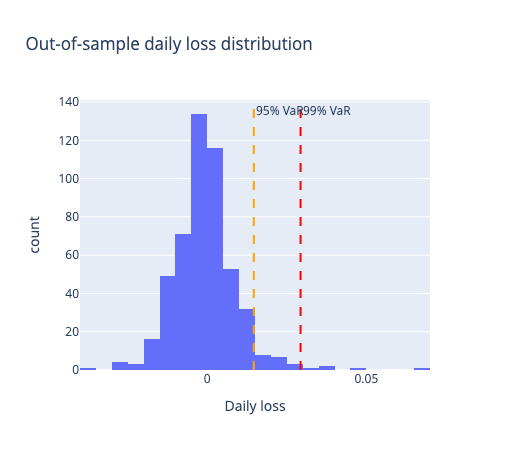
\includegraphics[width=0.85\linewidth]{out-of-sample-daily-loss-distribution.png}
  \caption{Out-of-sample daily loss distribution with 95\% and 99\% Value at Risk thresholds}
  \label{fig:out-of-sample-daily-loss-distribution}
\end{figure}

\subsection{Monte Carlo simulation}

Finally, a forecast-based evaluation apprach were used to asset expected return using Monte Carlo simulation. We simulated asset returns using in-sample annulaised expected return and covariance matrix, to preserve dependency between the portfolio assets across 252 trading days.

\begin{figure}[H]
  \centering
  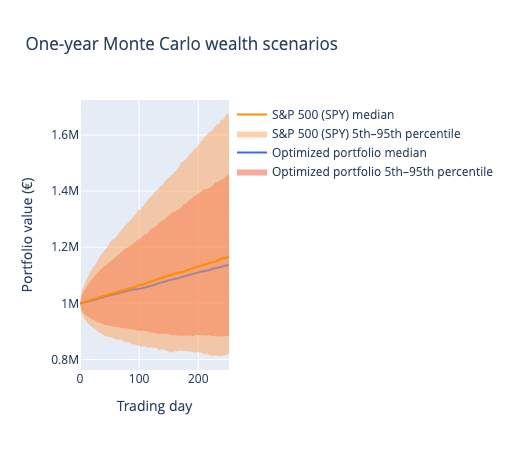
\includegraphics[width=0.85\linewidth]{one-year-monte-carlo-wealth-scenarios.png}
  \caption{One-year Monte Carlo wealth scenarios for the optimised portfolio and S\&P 500 benchmark}
  \label{fig:one-year-monte-carlo-wealth-scenarios}
\end{figure}

% =============================================================================
\section{Three Investor Scenarios and Results}
\label{sec:concrete-run}

% This section contains evidence; the preceding sections contain methods.

\subsection{Scenario definitions and common assumptions}

We perfomed senstivity analysis using three investor scenarios, demonstrating different views from risk point of view. (i) Risky investor emphasis growth over value, (ii) balanced investor combine growth and capital preservation, and conservative investor prioritise capital preservation and liquity over growth. Each scenario begins with \EUR1 million and uses the same asset universe, euro-denominated market data, estimation window, portfolio constraints methodology, and S\&P 500 benchmark. Table ~\ref{tab:scenario-profiles} showes the three investor outlook against the five questionnaire attribute.

\begin{table}[H]
  \centering
  \small
  \caption{Investor-scenario questionnaire responses}
  \label{tab:scenario-profiles}
  \begin{tabular}{p{0.29\linewidth}ccc}
    \toprule
    Questionnaire attribute & Risky & Balanced & Conservative \\
    \midrule
    Risk tolerance & Very high & Moderate & Low \\
    Investment horizon & Very long & Medium & Short \\
    Growth objective & Very high & Medium & Low \\
    Capital preservation & Low & Medium & High \\
    Liquidity requirement & Low & Medium & High \\
    \bottomrule
  \end{tabular}
\end{table}

\subsection{Phase I results: investor risk assessment}

The outcome of the first phase, highlight different investor risk score with the highest value attributed to the most risky invesotr portofilio and $\lambda$ of 1, and progress accordingly for balanced and conservative investors, as shown in Table~\ref{tab:scenario-risk-results}.

\begin{table}[H]
  \centering
  \caption{Investor risk results by scenario}
  \label{tab:scenario-risk-results}
  \begin{tabular}{lccc}
    \toprule
    Scenario & Risk score $R_Q$ & Risk profile & $\lambda$ \\
    \midrule
    Risky investor & 0.950 & Aggressive & 1 \\
    Balanced investor & 0.500 & Moderate & 5 \\
    Conservative investor & 0.250 & Conservative & 8 \\
    \bottomrule
  \end{tabular}
\end{table}

\subsection{Phase II results: suitability and asset-class allocation}

In phase II, the three sets of suitability scores are normalised separately across the available asset classes. This produces scenario-specific strategic allocations while ensuring that the asset-class weights for each investor sum to 100\% as showen in Table~\ref{tab:scenario-asset-class-allocation}.

\begin{table}[H]
  \centering
  \caption{Target asset-class weights by investor scenario}
  \label{tab:scenario-asset-class-allocation}
  \begin{tabular}{lccc}
    \toprule
    Asset class & Risky & Balanced & Conservative \\
    \midrule
    Equity & 30.96\% & 18.37\% & 10.09\% \\
    Fixed income & 12.48\% & 26.02\% & 33.21\% \\
    Cash & 6.32\% & 23.09\% & 34.31\% \\
    Real estate & 26.26\% & 17.40\% & 11.56\% \\
    Commodity & 23.99\% & 15.12\% & 10.83\% \\
    \midrule
    Total & 100\% & 100\% & 100\% \\
    \bottomrule
  \end{tabular}
\end{table}

We can see patterns arrise based on the expected return for each of the asset class. Fixed Income and Cash assets tend to increase monotonically from risky to conservative profiles, while Equity, Real estate, and Commodity move in oopposite direction.

\subsection{Phase III results: common market-data estimates}

The market-data inputs are held constant. The downloaded sample extends from 7-years for the whole dataset from October 2019 to October 2026. After calculating euro-denominated daily returns, the in-sample period contains 1,257 common observations for period of 5-years. The out-of-sample period contains 501 price observations from 2-years.

Asset universe has been defined capturing 119 instruments belong to the five modelled asset classes and possess the data required by the optimiser. Their in-sample annualised returns, volatilities, and covariance matrix are used unchanged for all three investors.

\subsection{Phase IV results: portfolio construction and optimisation}

\subsubsection{Risky investor portfolio}

The risky portfolio selects nine ETFs. The largest positions are BNO, SMH, SOXX, and XLRE at the 15\% security cap, followed by JNK at 12.48\%, VNQ at 11.26\%, SLV at 8.99\%, BIL at 6.32\%, and ARGT at 0.96\%. The allocation therefore uses commodities, semiconductor equities, listed real estate, and high-yield credit to target growth. It has an in-sample expected annual return of 17.59\%, volatility of 21.66\%, variance of 0.0469, and Sharpe ratio of 0.812.

\subsubsection{Balanced investor portfolio}

The balanced portfolio selects eleven ETFs. BIL receives 23.09\%, while SMH, XLRE, and SCHP each receive 15\%. The remaining allocation is distributed across VGSH (8.56\%), IAU (6.53\%), DBA (5.90\%), ARGT (3.37\%), BNO (2.69\%), TIP (2.45\%), and VNQ (2.40\%). The combination of Treasury bills, inflation-linked bonds, equities, real estate, and commodities reflects the investor's mixed growth and preserve capital objective. Expected annual return is 11.01\%, volatility is 12.72\%, variance is 0.0162, and the Sharpe ratio is 0.865.

\subsubsection{Conservative investor portfolio}

The conservative portfolio selects ten ETFs and assigns 34.31\% to BIL. SCHP and VGSH each receive 15\%, followed by XLRE at 11.56\%, SMH at 10.09\%, DBA at 5.58\%, IAU at 3.89\%, VCSH at 3.21\%, BNO at 1.29\%, and CPER at 0.06\%. Cash and short-duration or inflation-linked fixed income dominate the allocation, although smaller growth and real-asset exposures maintain diversification across. Expected annual return is 7.54\%, volatility is 9.80\%, variance is 0.0096, and the Sharpe ratio is 0.769.

Table~\ref{tab:scenario-optimized-summary} summarise the expected annual return, volatile, variance, sharp ratio and number of holdings.

\begin{table}[H]
  \centering
  \small
  \caption{Optimised in-sample portfolio characteristics by scenario}
  \label{tab:scenario-optimized-summary}
  \begin{tabular}{lccc}
    \toprule
    Metric & Risky & Balanced & Conservative \\
    \midrule
    Expected annual return & 17.59\% & 11.01\% & 7.54\% \\
    Annualised volatility & 21.66\% & 12.72\% & 9.80\% \\
    Variance & 0.0469 & 0.0162 & 0.0096 \\
    Sharpe ratio & 0.812 & 0.865 & 0.769 \\
    Number of holdings & 9 & 11 & 10 \\
    \bottomrule
  \end{tabular}
\end{table}

\subsection{Phase V results: benchmarking and performance analysis}

\subsubsection{Out-of-sample performance}

We perform out-of-samople for 2-years over the three investor profiles, the risky portfolio outperform SPY, market proxy benchmark. The balanced portfolio tracked SPY but finished slightly below SPY, while the conservative portfolio finished significantly below SPY, All the three portfolios achieve a higher Sharpe ratio than the benchmark, although the comparison is specific to this two-year sample. Figure~\ref{tab:scenario-performance} shows the three portfolios over the 2-years starting with \EUR1 million.

\begin{table}[H]
  \centering
  \small
  \caption{Out-of-sample performance by investor scenario}
  \label{tab:scenario-performance}
  \begin{tabular}{lrrrr}
    \toprule
    Metric & Risky & Balanced & Conservative & S\&P 500 (EUR) \\
    \midrule
    Total return & 70.56\% & 32.71\% & 22.53\% & 36.10\% \\
    Annualised return & 30.67\% & 15.23\% & 10.72\% & 16.70\% \\
    Annualised volatility & 21.03\% & 12.22\% & 9.79\% & 17.88\% \\
    Sharpe ratio & 1.458 & 1.247 & 1.095 & 0.934 \\
    Maximum drawdown & 20.87\% & 13.08\% & 12.09\% & 23.03\% \\
    Ending value & \EUR1,705,595 & \EUR1,327,058 & \EUR1,225,349 & \EUR1,360,970 \\
    \bottomrule
  \end{tabular}
\end{table}

\begin{figure}[H]
  \centering
  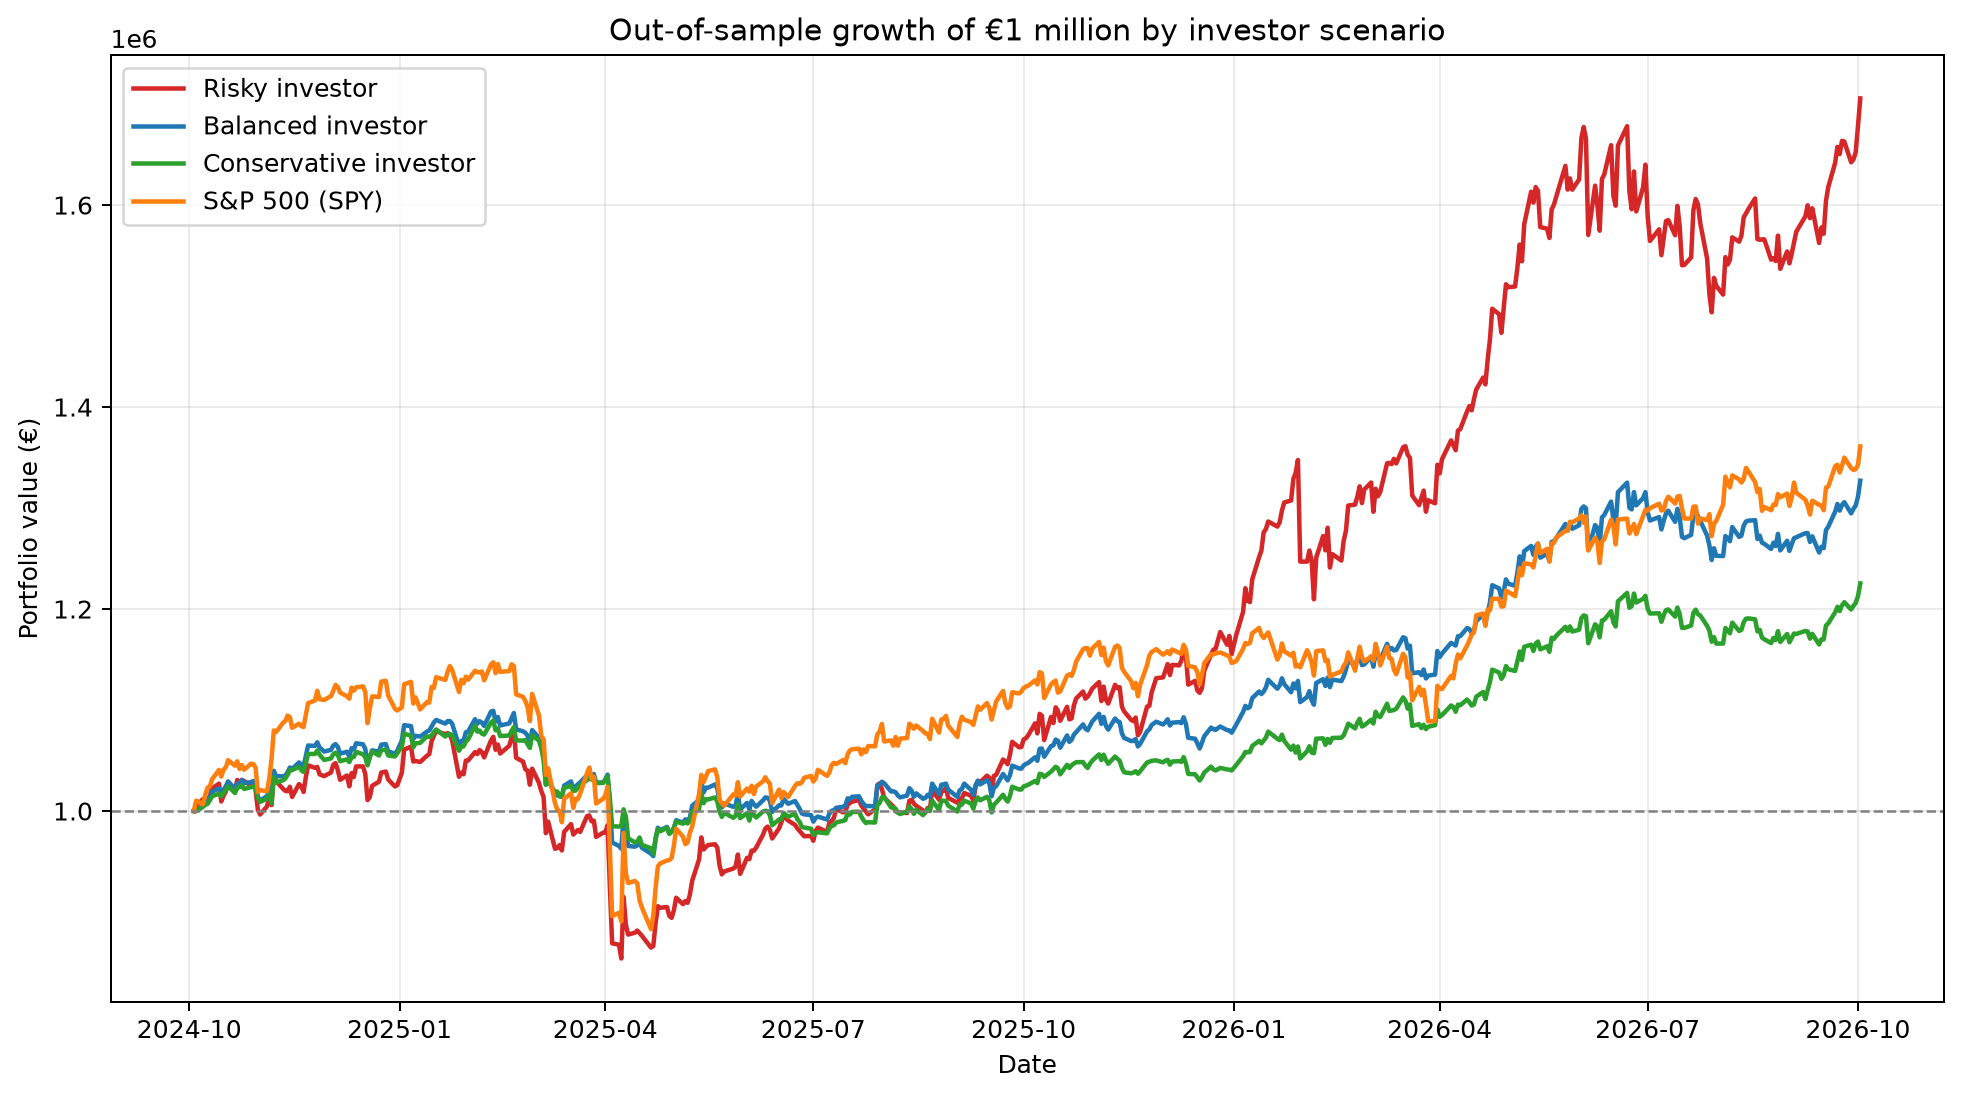
\includegraphics[width=0.9\linewidth]{three-scenario-out-of-sample-growth.png}
  \caption{Growth of \EUR1 million: three optimised investor portfolios versus the S\&P 500}
  \label{fig:scenario-holdout-growth}
\end{figure}

\subsubsection{Downside-risk results}

At the 95\% confidence level, the loss thresholds on \EUR1 million are approximately \EUR21,864, \EUR12,359, and \EUR9,241 for the risky, balanced, and conservative portfolios, respectively. Corresponding Expected Shortfalls are approximately \EUR33,160, \EUR17,696, and \EUR13,740.

As expected, the risky portfolio has greater tail exposure than SPY, whereas both the balanced and conservative portfolios reduce VaR and ES at both confidence levels. Table~\ref{tab:scenario-tail-risk} showes out-of-sample historical one-day VaR and ES.

\begin{table}[H]
  \centering
  \small
  \caption{Out-of-sample historical one-day VaR and Expected Shortfall}
  \label{tab:scenario-tail-risk}
  \begin{tabular}{lrrrr}
    \toprule
    Strategy & 95\% VaR & 95\% ES & 99\% VaR & 99\% ES \\
    \midrule
    Risky & 2.19\% & 3.32\% & 3.86\% & 5.85\% \\
    Balanced & 1.24\% & 1.77\% & 2.35\% & 2.97\% \\
    Conservative & 0.92\% & 1.37\% & 2.12\% & 2.31\% \\
    S\&P 500 (EUR) & 1.64\% & 2.63\% & 3.30\% & 4.73\% \\
    \bottomrule
  \end{tabular}
\end{table}

\subsubsection{Monte Carlo simulation results}

Finally, applying Monte Carlo simulation, the risky portfolio has the highest median wealth, but its 5th percentile is lower than those of the balanced and conservative portfolios. The conservative portfolio has the highest 5th-percentile wealth, indicating stronger downside protection, while retaining the lowest upside, as shown in Table~\ref{tab:scenario-simulation}.

\begin{table}[H]
  \centering
  \small
  \caption{One-year Monte Carlo terminal-wealth results}
  \label{tab:scenario-simulation}
  \begin{tabular}{lrrr}
    \toprule
    Strategy & Median & 5th percentile & 95th percentile \\
    \midrule
    Risky & \EUR1,161,882 & \EUR820,441 & \EUR1,657,255 \\
    Balanced & \EUR1,108,812 & \EUR897,039 & \EUR1,364,307 \\
    Conservative & \EUR1,073,354 & \EUR912,024 & \EUR1,259,734 \\
    S\&P 500 (EUR) & \EUR1,160,958 & \EUR812,040 & \EUR1,666,150 \\
    \bottomrule
  \end{tabular}
\end{table}

% =============================================================================
\section{Conclusion}
\label{sec:conclusion}

In thie report, we discussed an end-to-end framework for constructing and evaluating portfolio based on set of investor's key attributes. The framework link investor preference to portfolio decisions through five phases: investor risk assessment, asset-class suitability, market-data preparation, security-level optimisation, and out-of-sample performance evaluation. Three investor scenarios were examined as a broad senstivity analysis for the in-sample dataset, The risky investor received the highest allocation to equities, real estate, and commodities, producing the highest expected return but also the greatest volatility and tail risk. The conservative investor received the largest allocation to cash and fixed income, resulting in the lowest volatility, drawdown, VaR, and Expected Shortfall. The balanced portfolio occupied the middle ground and provided a more even compromise between growth and capital preservation.

% =============================================================================

\clearpage
\appendix

\clearpage
\begin{landscape}
  \section{Full Asset Universe}
  \label{app:full-asset-universe}

  This appendix reproduces the complete asset universe from \texttt{asset\_universe.csv}.

  \IfFileExists{../asset_universe.csv}
  {\def\AssetUniverseFile{../asset_universe.csv}}
  {\def\AssetUniverseFile{asset_universe.csv}}

  \scriptsize
  \setlength{\tabcolsep}{3pt}
  \csvreader[
    respect all,
    longtable={>{\raggedright\arraybackslash}p{0.07\linewidth}>{\raggedright\arraybackslash}p{0.27\linewidth}>{\raggedright\arraybackslash}p{0.07\linewidth}>{\raggedright\arraybackslash}p{0.12\linewidth}>{\raggedright\arraybackslash}p{0.22\linewidth}>{\raggedright\arraybackslash}p{0.15\linewidth}},
    table head={
      \caption{Complete investable asset universe}\label{tab:full-asset-universe}\\
      \toprule
      Ticker & Display name & Type & Asset class & Asset subclass & Geography \\
      \midrule
      \endfirsthead
      \caption[]{Complete investable asset universe (continued)}\\
      \toprule
      Ticker & Display name & Type & Asset class & Asset subclass & Geography \\
      \midrule
      \endhead
      \midrule
      \multicolumn{6}{r}{Continued on next page}\\
      \endfoot
      \bottomrule
      \endlastfoot
    },
    late after line=\\
  ]{\AssetUniverseFile}
  {ticker=\Ticker,display_name=\DisplayName,instrument_type=\InstrumentType,asset_class=\AssetClass,asset_subclass=\AssetSubclass,geography=\Geography}
  {\Ticker & \DisplayName & \InstrumentType & \AssetClass & \AssetSubclass & \Geography}
\end{landscape}

\section{Reproducibility}

\begin{itemize}
  \item Notebook: \texttt{FIN42350 Portfolio Design Project.ipynb}
  \item Asset universe: \texttt{data/asset\_universe.csv}
  \item Dashboard application: \texttt{source/portfolio.py}
\end{itemize}

\end{document}
